%%%%%%%%%%%%%%%%%%%%%%%%%%%%%%%%%%%%%%%%
%% MCM/ICM LaTeX Template %%
%% 2023 MCM/ICM           %%
%%%%%%%%%%%%%%%%%%%%%%%%%%%%%%%%%%%%%%%%
\documentclass[12pt]{article}
\usepackage{geometry}
\geometry{left=1in,right=0.75in,top=1in,bottom=1in}

%%%%%%%%%%%%%%%%%%%%%%%%%%%%%%%%%%%%%%%%
% Replace ABCDEF in the next line with your chosen problem
% and replace 1111111 with your Team Control Number
\newcommand{\Problem}{A}
\newcommand{\Team}{2303965}
%%%%%%%%%%%%%%%%%%%%%%%%%%%%%%%%%%%%%%%%

\usepackage{newtxtext}
\usepackage{amsmath,amssymb,amsthm}
\usepackage{newtxmath} % must come after amsXXX
\usepackage{booktabs}
\usepackage[pdftex]{graphicx}
\usepackage{xcolor}
\usepackage{fancyhdr}
\usepackage{cite} 
\usepackage[inkscapelatex=false]{svg}
\usepackage{subfigure}

\lhead{Team \Team}
\rhead{}
\cfoot{}

\newtheorem{theorem}{Theorem}
\newtheorem{corollary}[theorem]{Corollary}
\newtheorem{lemma}[theorem]{Lemma}
\newtheorem{definition}{Definition}


%%%%%%%%%%%%%%%%%%%%%%%%%%%%%%%%
\begin{document}

\graphicspath{{.}}  % Place your graphic files in the same directory as your main document
\DeclareGraphicsExtensions{.pdf, .jpg, .tif, .png}
\thispagestyle{empty}
\vspace*{-16ex}
% \centerline{\begin{tabular}{*3{c}}
% 		\parbox[t]{0.3\linewidth}{\begin{center}\textbf{Problem Chosen}\\ \Large \textcolor{red}{\Problem}\end{center}}
% 		 & \parbox[t]{0.3\linewidth}{\begin{center}\textbf{2023\\ MCM/ICM\\ Summary Sheet}\end{center}}
% 		 & \parbox[t]{0.3\linewidth}{\begin{center}\textbf{Team Control Number}\\ \Large \textcolor{red}{\Team}\end{center}} \\
% 		\hline
% 	\end{tabular}}
%%%%%%%%%%% Begin Summary %%%%%%%%%%%
% Enter your summary here replacing the (red) text
% Replace the text from here ...
\vspace{0.5cm}

\begin{center}
	\LARGE \textbf{How many plants can hit a drought?\\ One or two more?}
\end{center}

\vspace{0.5cm}

"Global temperatures are warming, glaciers are melting, sea levels are rising,..." All parts of the world are facing huge environmental disasters. In recent years, unusual weather and climate events have become more and more intense, and the number of "record-breaking" extreme weather events has increased. Trees are also becoming thin and weak under drought conditions. How many plants can survive drought conditions without being defeated and become the last survivors? 

In this paper, we investigate the change of species biomass over time under irregular weather conditions. For this we developed the \textbf{Plant Community Interaction Model} and an {Improved Logistic Growth Competition Model}. By using these two models, we investigated the tolerance of plant species and populations to the environment under drought conditions.

First, we obtained a series of time-series images through the US nasa and worldview websites, and preprocessed the data through \textbf{data visualization} and \textbf{cubic spline interpolation}. In order to predict the changes of anomalous weather cycles and species populations, we developed the Lotka-Volterra competition model, further introduced the associated competition and growth coefficients, and derived a plot of actual species biomass versus time by analyzing the effects of their interspecific relationships on environmental biomass. In addition, we also proposed the climatic factors affecting environmental biomass, and selected the three most influential factors, temperature, precipitation and light, to derive the predicted species biomass versus time, and then determined the weight of each factor by \textbf{difference fitting} and \textbf{entropy weight-multiple linear regression}, and finally we obtained the predictive model of species biomass over time during the drought cycle.

Second, to explore the relationship of how species species benefit the community. We selected three species with the same climate in the ecosystem as the study object and proposed an \textbf{Improved Logistic Growth Competition Model}. Based on this, we introduced the drought factor and species contact coefficients by considering environmental effects and interspecies effects, and the species contact coefficients were calculated separately. In the study of community benefit, we considered two parameters, Fraction of Photosynthetically Active Radiation and Gross Primary Productivity, to evaluate the impact brought by the ecosystem, and finally obtained the functional relationship between the species contact coefficient and the benefit coefficient by fitting the function Finally, the functional relationship between the species exposure coefficient and the benefit coefficient was obtained by fitting the function. The minimum number of species to benefit the community was determined to be \textbf{460} when the species contact coefficient was \textbf{0.00937}.

Finally, we tested the robustness and sensitivity of the Improved Logistic Growth Competition Model and found that the model had better sensitivity by varying the images obtained from the species contact coefficients. We also evaluated the strengths and weaknesses of the model.

\vspace{0.5cm}

\textbf{Keywords:} \textit{Lotka-Volterra competition model, improved logistic growth competition model, data visualization}

% to here
%%%%%%%%%%% End Summary %%%%%%%%%%%

%%%%%%%%%%%%%%%%%%%%%%%%%%%%%%
\clearpage
\pagestyle{fancy}
% Uncomment the next line to generate a Table of Contents

\tableofcontents

\newpage
\setcounter{page}{1}
\rhead{Page \thepage\ }
%%%%%%%%%%%%%%%%%%%%%%%%%%%%%% 
\section{Introduction}

\subsection{Problem Background}

Since plants can only grow in their pristine environment, they are vulnerable to various abiotic environmental impacts of stress such as sunlight, temperature, humidity, and drought throughout their growth and development. As one of the major abiotic stresses that affect normal plant growth and development and limit plant community diversity, drought affects plant life activities such as growth, development, and reproduction. Different species respond differently to their environment, while drought environments vary in their alteration of species traits. What is the minimum number of species required for a plant community to benefit from this local biodiversity? How does this phenomenon expand as the number of species increases? What does this imply for the long-term viability of plant communities?

\begin{figure}[htb]
	\centering
	\subfigure[Mountains]{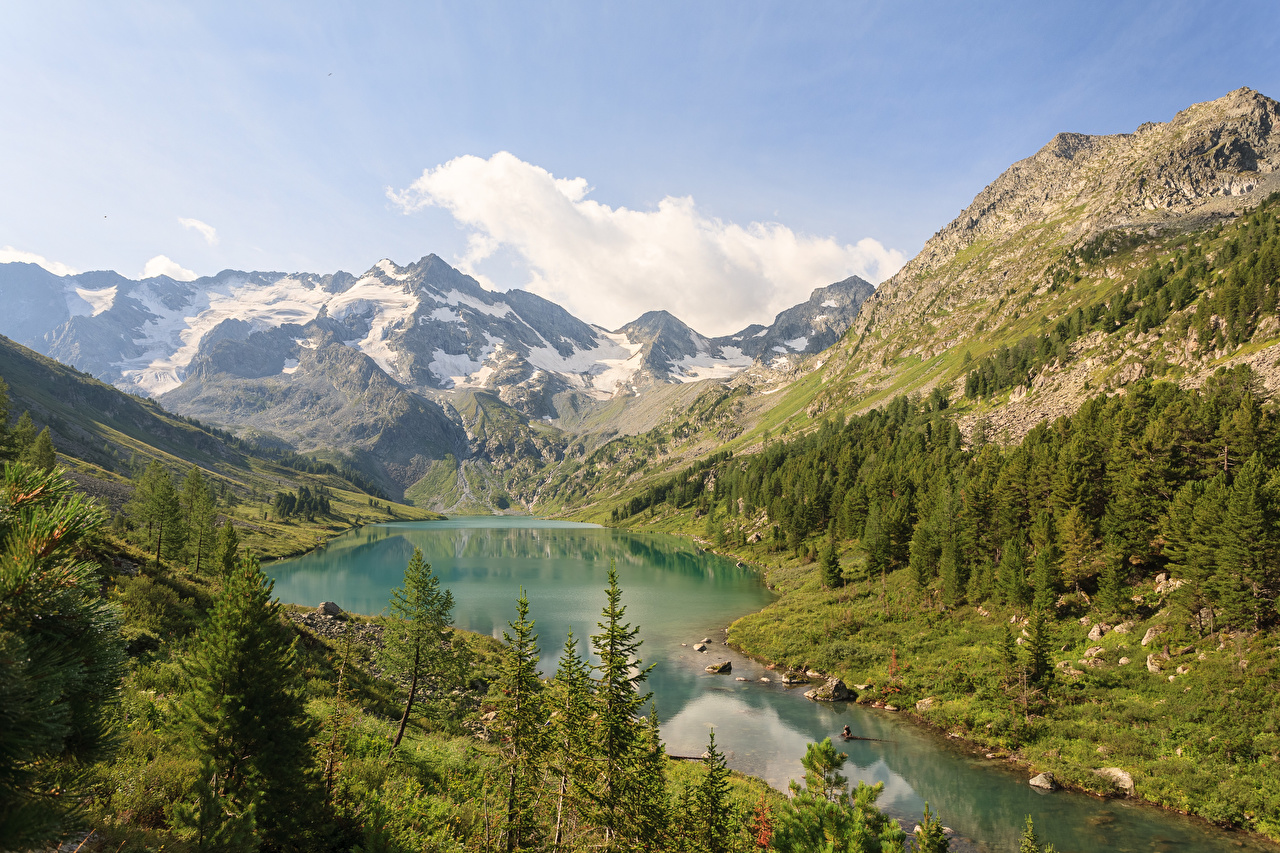
\includegraphics[width=0.3\textwidth]{Mountains_Lake_Forests_Russia_Chui_Lake_Altai_613981_1280x853.jpg}}
	\subfigure[Grasslands]{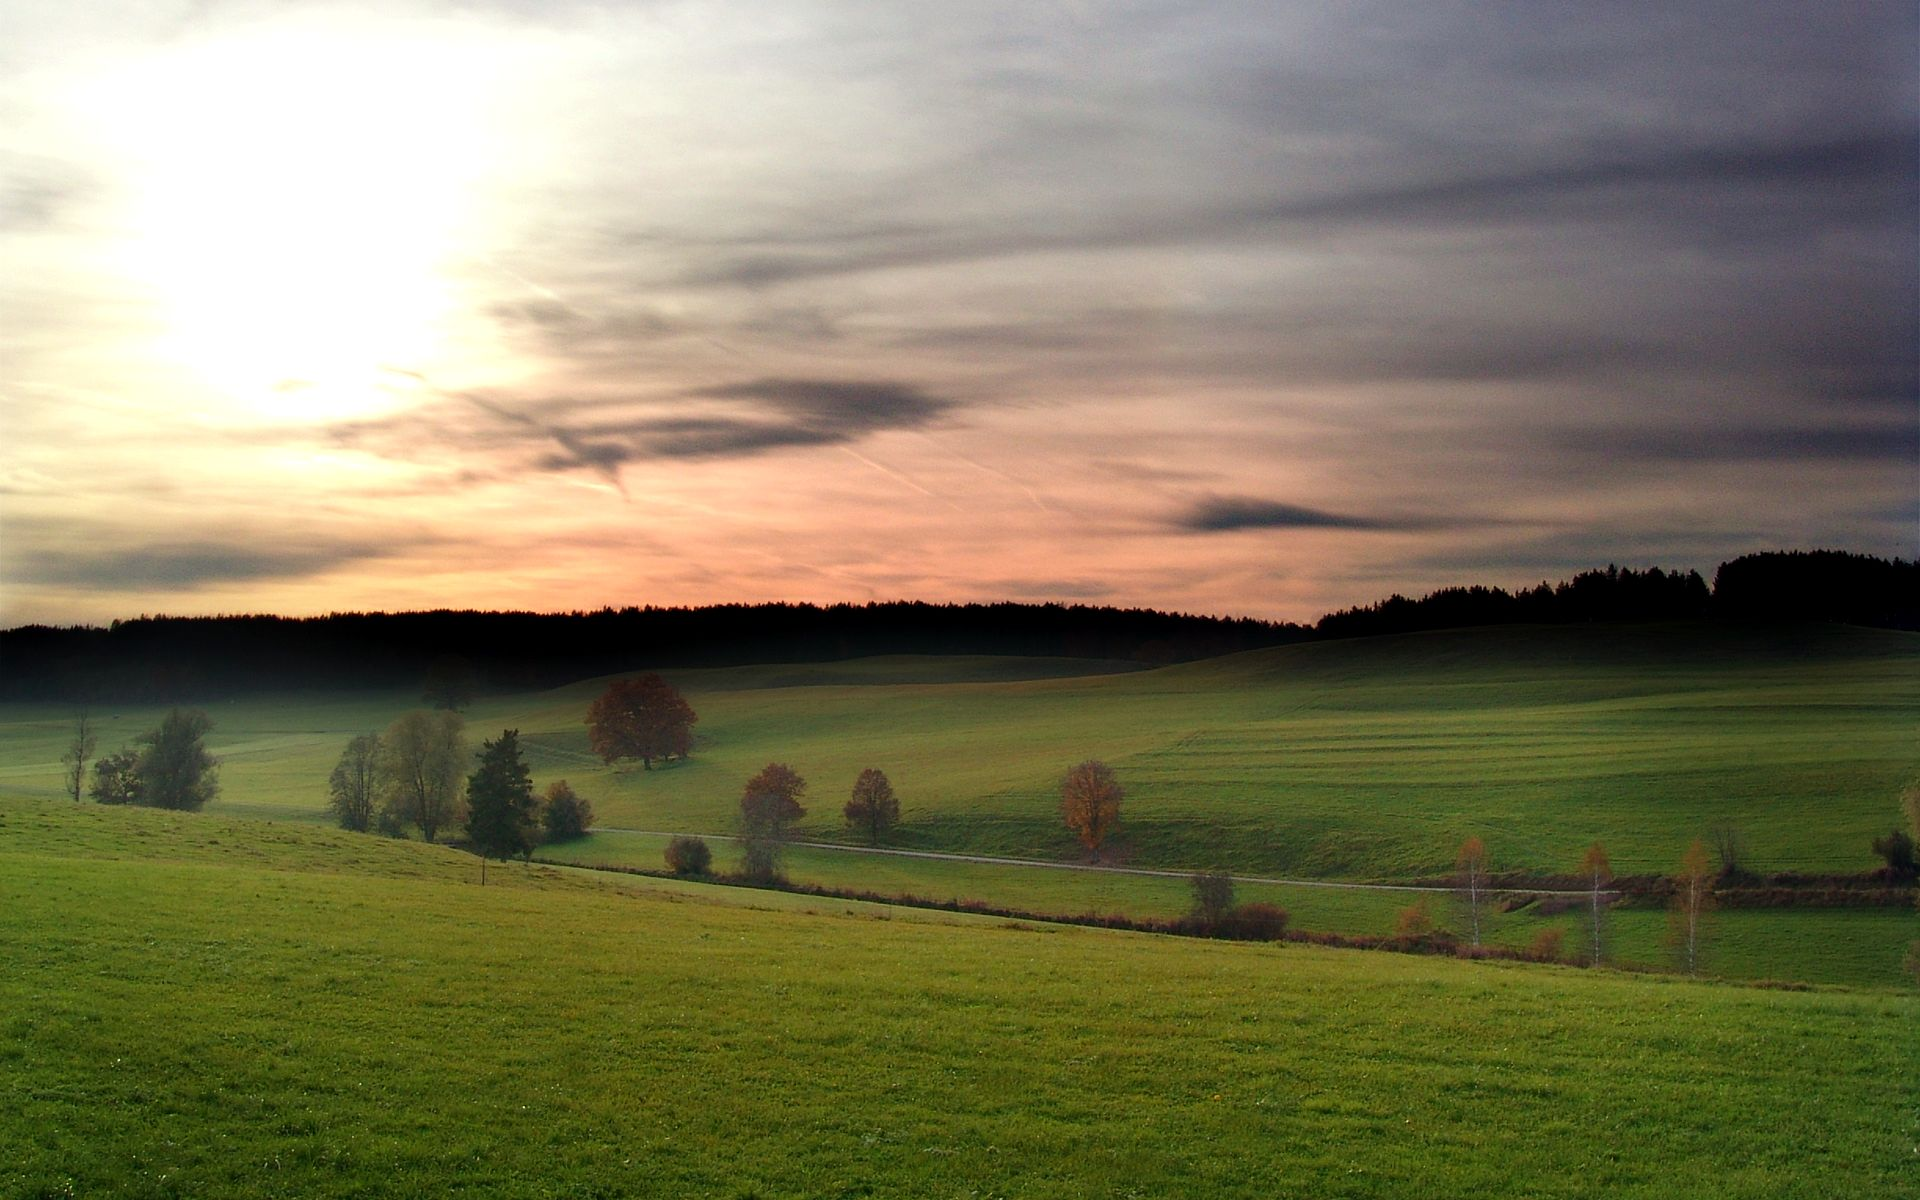
\includegraphics[width=0.3\textwidth]{173138-Sepik.jpg}}
	\subfigure[Dessert]{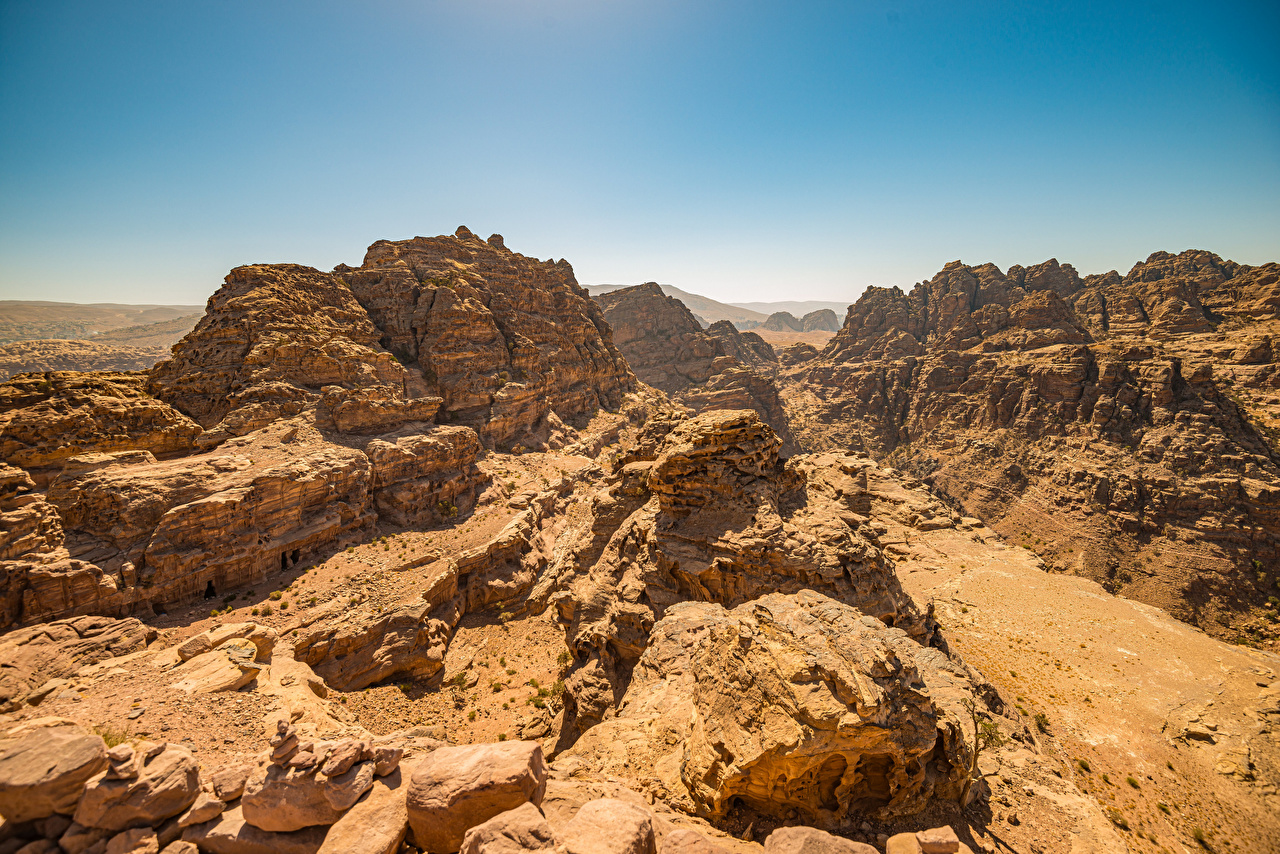
\includegraphics[width=0.3\textwidth]{Desert_Petra_Jordan_Crag_591491_1280x854.jpg}}
	\caption{Plant communities in different environments.}
\end{figure}

\subsection{Restatement of Problem}

Considering the background information of plant and limiting conditions identified in the Problem Background , the main tasks of this paper are as follows:

\begin{enumerate}
	\item A mathematical model is developed for predicting trends in plant communities over time in the face of irregular weather cycles. For example, in periods of drought when rain is supposed to fall, we will consider the interspecific relationships of plants to better predict changes in plant community biodiversity.
	\item With environmental variations, the sensitivity of different plant species to these changes may also vary. When the number of species increases, the ecosystem of the plant community may change, including species competition, interactions, etc., which in turn affects the ecological balance of the plant community.
	\item Evaluate and predict the role and importance of species diversity for the ecosystems in which the species lives.
	\item Future droughts occurring with greater frequency and variability will have widespread impacts on ecosystems and human societies. This could lead to water scarcity, poor crop yields, and increased desertification, thereby threatening biodiversity and human well-being.
	\item Pollution factors and habitat destruction are objectively present problems in the environment, which may significantly affect the conclusions. These problems may lead to loss of biodiversity, loss of ecosystem function, or even to the destruction of entire ecological chains.
	\item It is important to evaluate and predict the role and importance of species diversity to the ecosystem in which it is found. Species diversity is a key feature of ecosystems and has important implications for ecosystem health and stability.
\end{enumerate}

\subsection{Literature Review}

In recent years, the frequency of abnormal weather has increased significantly with global warming and human activities, and these abnormal weather events have had a dramatic impact on plant communities. It may affect the distribution range of species, and the composition of species and lead to changes in ecosystems. Thus, the analysis of the effects of the relationship between abnormal weather and plant populations has far-reaching implications for the succession of plant populations.

Clark, James S., et al. \cite{clark2016impacts} suggested that in the eastern United States, the effects of increased drought are better understood at the level of individual trees. Grossiord, Charlotte, et al. \cite{grossiord2014does} modeled the predicted climate impacts on biodiversity across the continental United States.

Tilman, D., Reich, P. B., et al. \cite{tilman2006biodiversity} discussed the high climate variability during the growing season over a decade, resulting in year-to-year changes in plant species abundance and ecosystem productivity. The greater the number of plant species, the greater the temporal stability of the annual production of above-ground plants in the ecosystem. Huang, W., Wang, W., et al. \cite{huang2021local}  studied the stability of grassland ecosystems under drought. concluded that alpine grasslands and alpine meadows were the most resistant but the least resilient. Meadow steppe and typical grassland were the least resistant but the most resilient.

Prugh, Laura R., et al. \cite{prugh2018ecological} responded that plants are most responsive to a year of water deficit under extreme drought conditions. Spinoni, Jonathan, et al. \cite{spinoni2014world} quantified the effects of extreme climatic events on contemporary ecological community composition.

Zvereva, Elena L., Eija Toivonen, and Mikhail V. Kozlov. \cite{zvereva2008changes} showed for the first time that there are geographical differences in plant community responses to air emissions. By investigating the effects of IAP on Italian plant communities and Natura 2000 habitats, Lazzaro, Lorenzo, et al. concluded that competition was the main mechanism of influence. \cite{lazzaro2020impact}


\subsection{Our work}

We need to analyze the laws behind the irregular weather and the effects between different species, and then build mathematical models based on them. In this paper, our work is focused on the following points:

\begin{itemize}
	\item Establishing Lotka-Volterra model based on multiple regression entropy weighting method, which can predict the results more accurately by the given input parameter values within a certain range.
	\item Predicting the effects of abnormal weather cycles and plant community biomass by analyzing the interspecific relationships of communities and the three factors affecting climate variables: temperature, precipitation, and light.
	\item Based on the above Lotka-Volterra model, a variety of factors including the environment is considered and parameters are added to make the model more responsive to the parameters and have better sensitivity.
	\item Successfully predicted the minimum number of species that would benefit itself from an ecosystem perspective.
	\item Discusses how to face drought in the future and makes recommendations from an ecosystem perspective
\end{itemize}

\section{Assumptions and Justifications}

\begin{itemize}
	\item \textbf{Assumption 1:} There is no significant effect on the community except for the influencing factors proposed in the text. \\
	      \textbf{Justification:} Nature is a chaotic system with many external changing conditions, such as soil moisture, rainfall rate, and ozone layer hole. In order to simplify our model, other than the factors mentioned in the text, other factors did not have significant effects on the community.

	\item \textbf{Assumption 2:} The variation of species biomass is determined by its internal and external factors, and the internal and external factors do not influence or interfere with each other. \\
	      \textbf{Justification:} Changes in species biomass are determined by both internal and external factors, and in order to make our model results strongly correlated with the factors that appear in the model, we consider that internal and external factors do not interfere with each other and only the factors that appear in the model need to be considered.

	\item \textbf{Assumption 3:} The competitiveness index of each species is assumed to be fixed for each period of biological competition.\\
	      \textbf{Justification:} Since the change in the number of species does not change its original competitive index at each stage of the biological competition, the competitive index can remain approximately constant at a fixed stage.

	\item \textbf{Assumption 4:} The data at the data collection sites represent the data of the whole region.\\
	      \textbf{Justification:} Since the climatic conditions of a region are roughly comparable, there may be a few points of difference, so we can assume that the climatic conditions of a region are roughly comparable.

	\item \textbf{Assumption 5:} The growth rate of species growth is assumed to be continuous and stable.\\
	      \textbf{Justification:} The growth rate of a species is continuous and stable according to its survival years and also the environment will affect its growth rate.
\end{itemize}

\section{Notation}

All symbols used in this paper are shown in Table \ref{tab:notation}

\begin{table}[]
	\centering
	\caption{Notation}
	\begin{tabular}{@{}ll@{}}
		\toprule                                        \\
		Symbols  & Definitions                          \\
		\midrule                                        \\
		$N$      & Number of individuals of the species \\
		$r$      & Species intrinsic growth rate        \\
		$K$      & Environmental capacity               \\
		$\alpha$ & Drought coefficient scale factor     \\
		$D$      & Drought coefficient                  \\
		$\beta$  & Species contact factor               \\
		$\delta$ & Standard deviation of the linear fit \\
		\bottomrule
	\end{tabular}
	\label{tab:notation}
\end{table}

\section{The Data}

\subsection{Data Collection}

Data collection plays a role in mathematical modeling. the data we use in the paper comes from two main sources, one of which is NASA's worldview. worldview provides data from several satellites, including Terra, Aqua, Suomi NPP, and NOAA. a worldview can be used to browse and analyze natural and anthropogenic activities on the Earth's surface, such as meteorological phenomena, fires, climate change, land, and ocean surface temperatures, etc. We use Python to capture and visualize all data from 2010-2020 into images, the visualized image obtained from the search is shown in Figure \ref{fig:visualization_satellites}.

\begin{figure}[htb]
	\centering
	\subfigure[Grasslands]{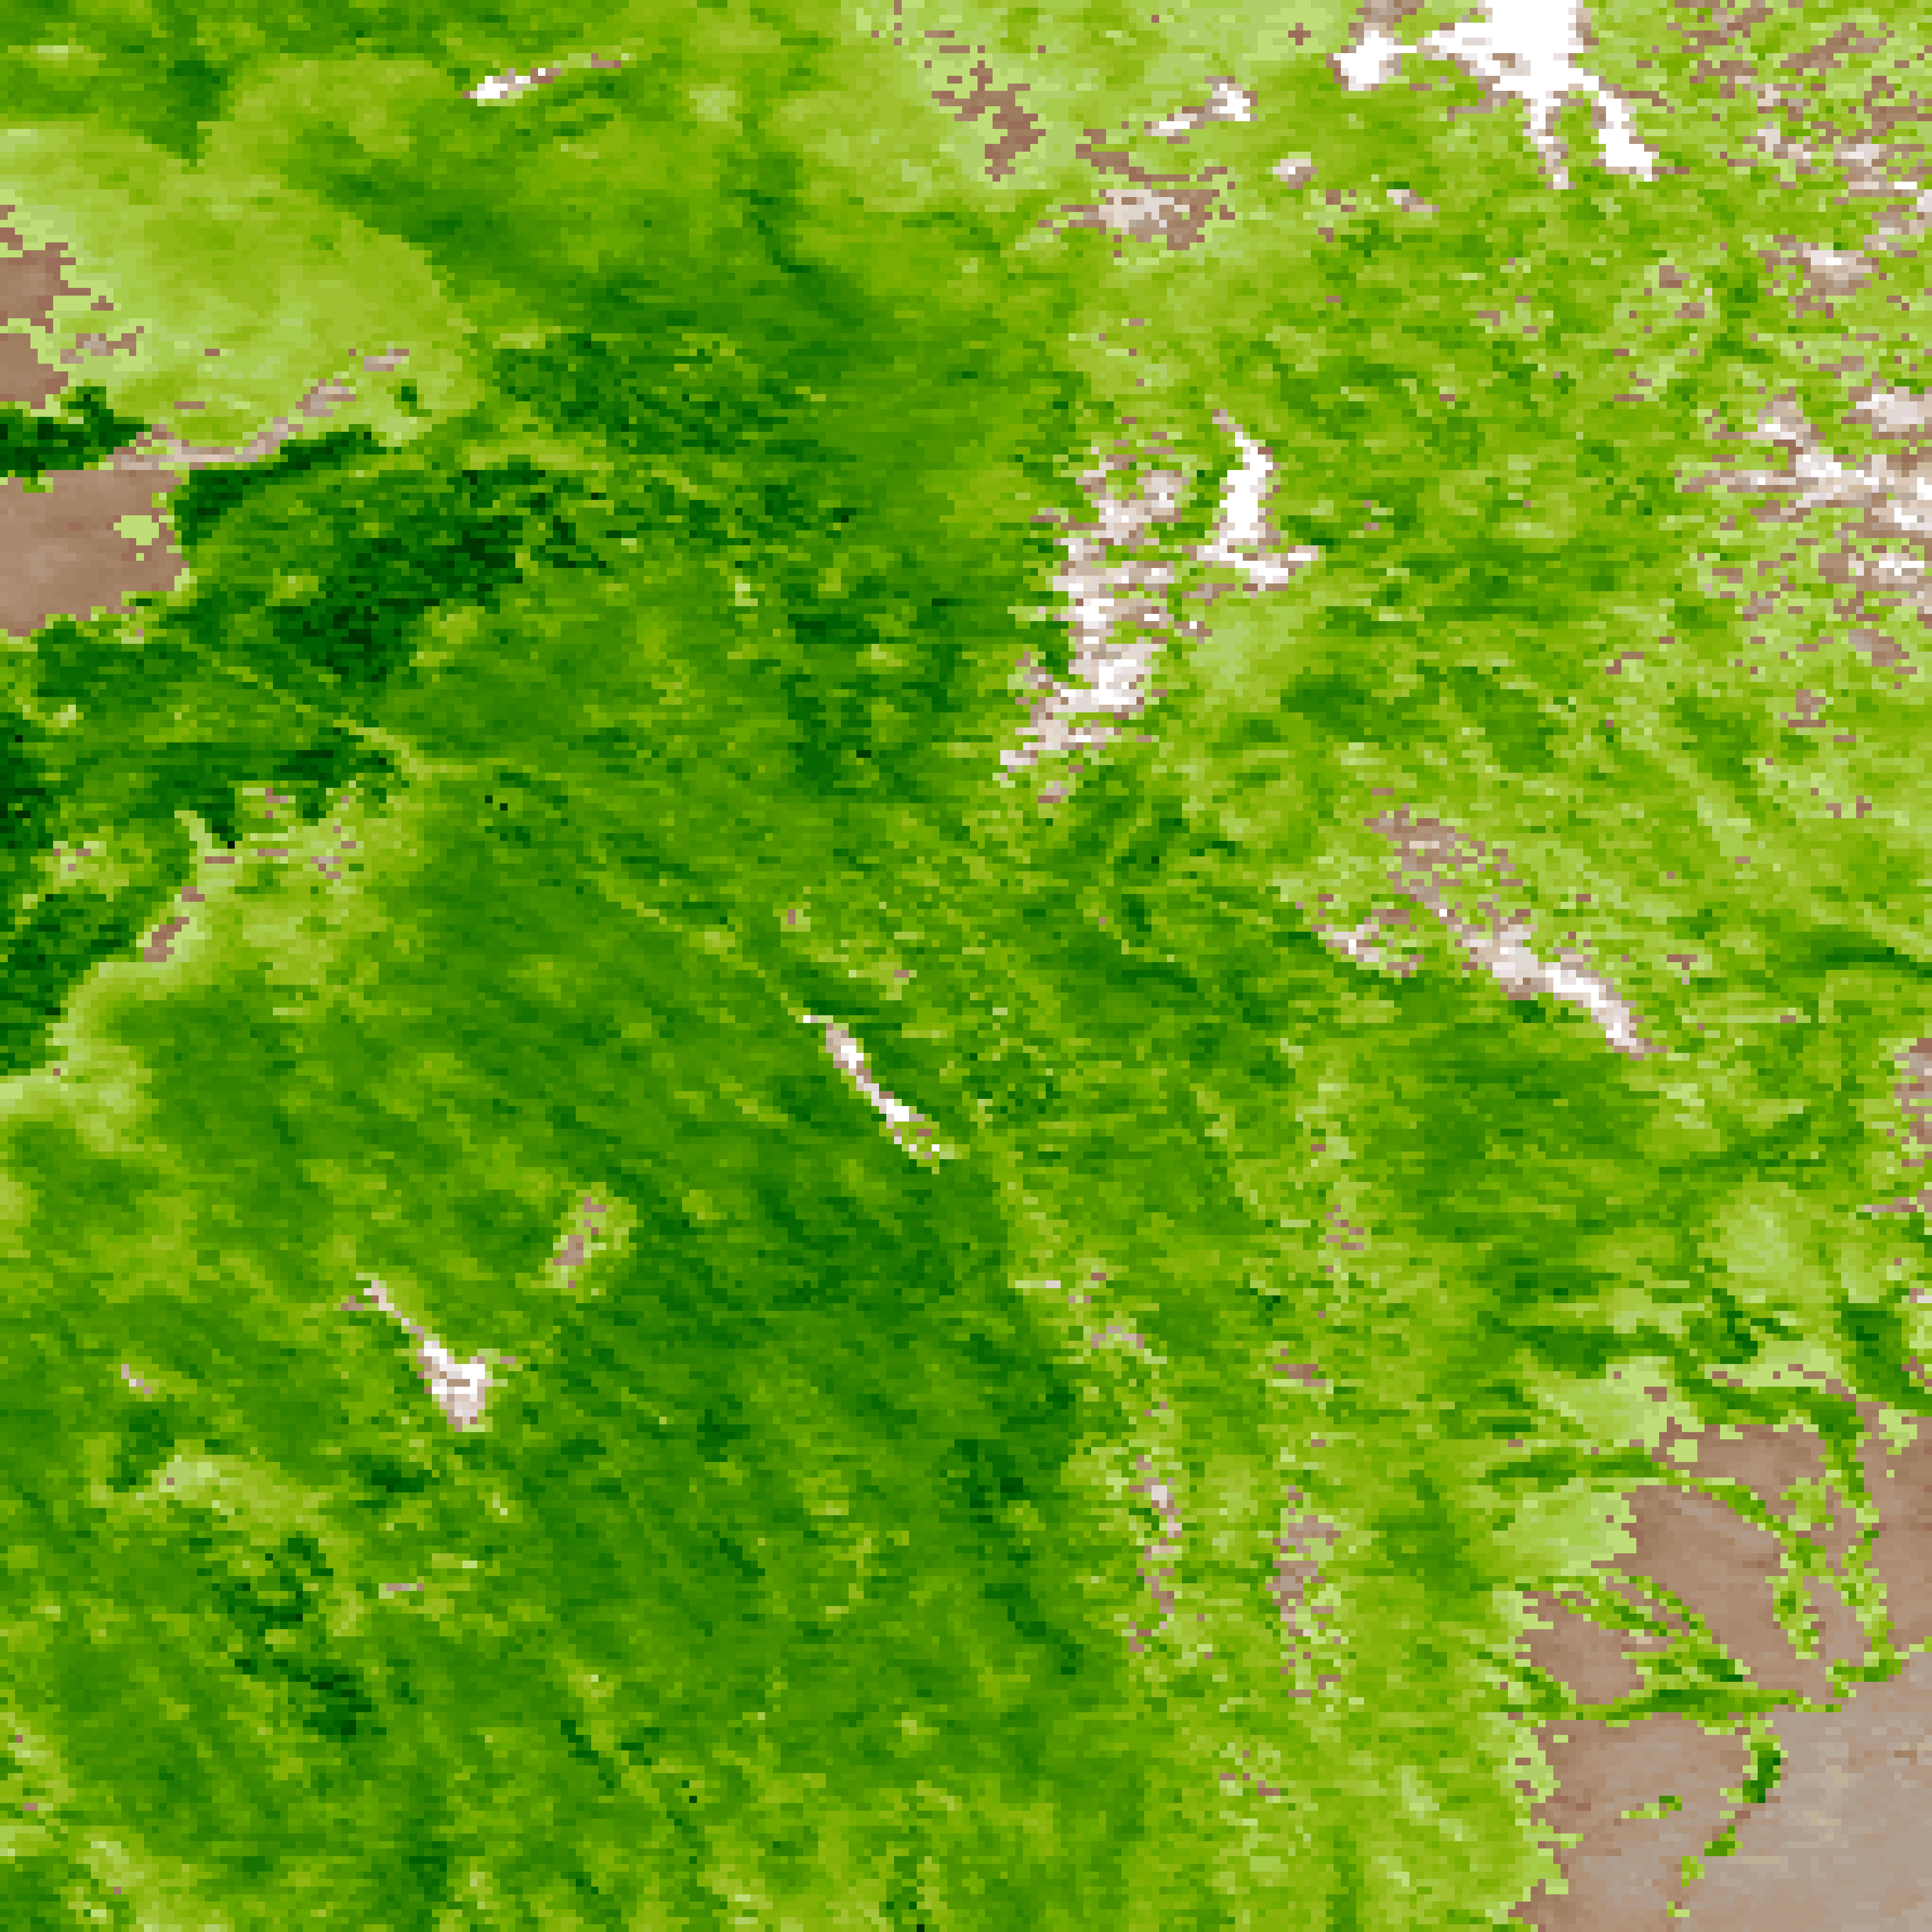
\includegraphics[width=2.5in]{download/grassland/20110725.png}}
	\subfigure[Temperature]{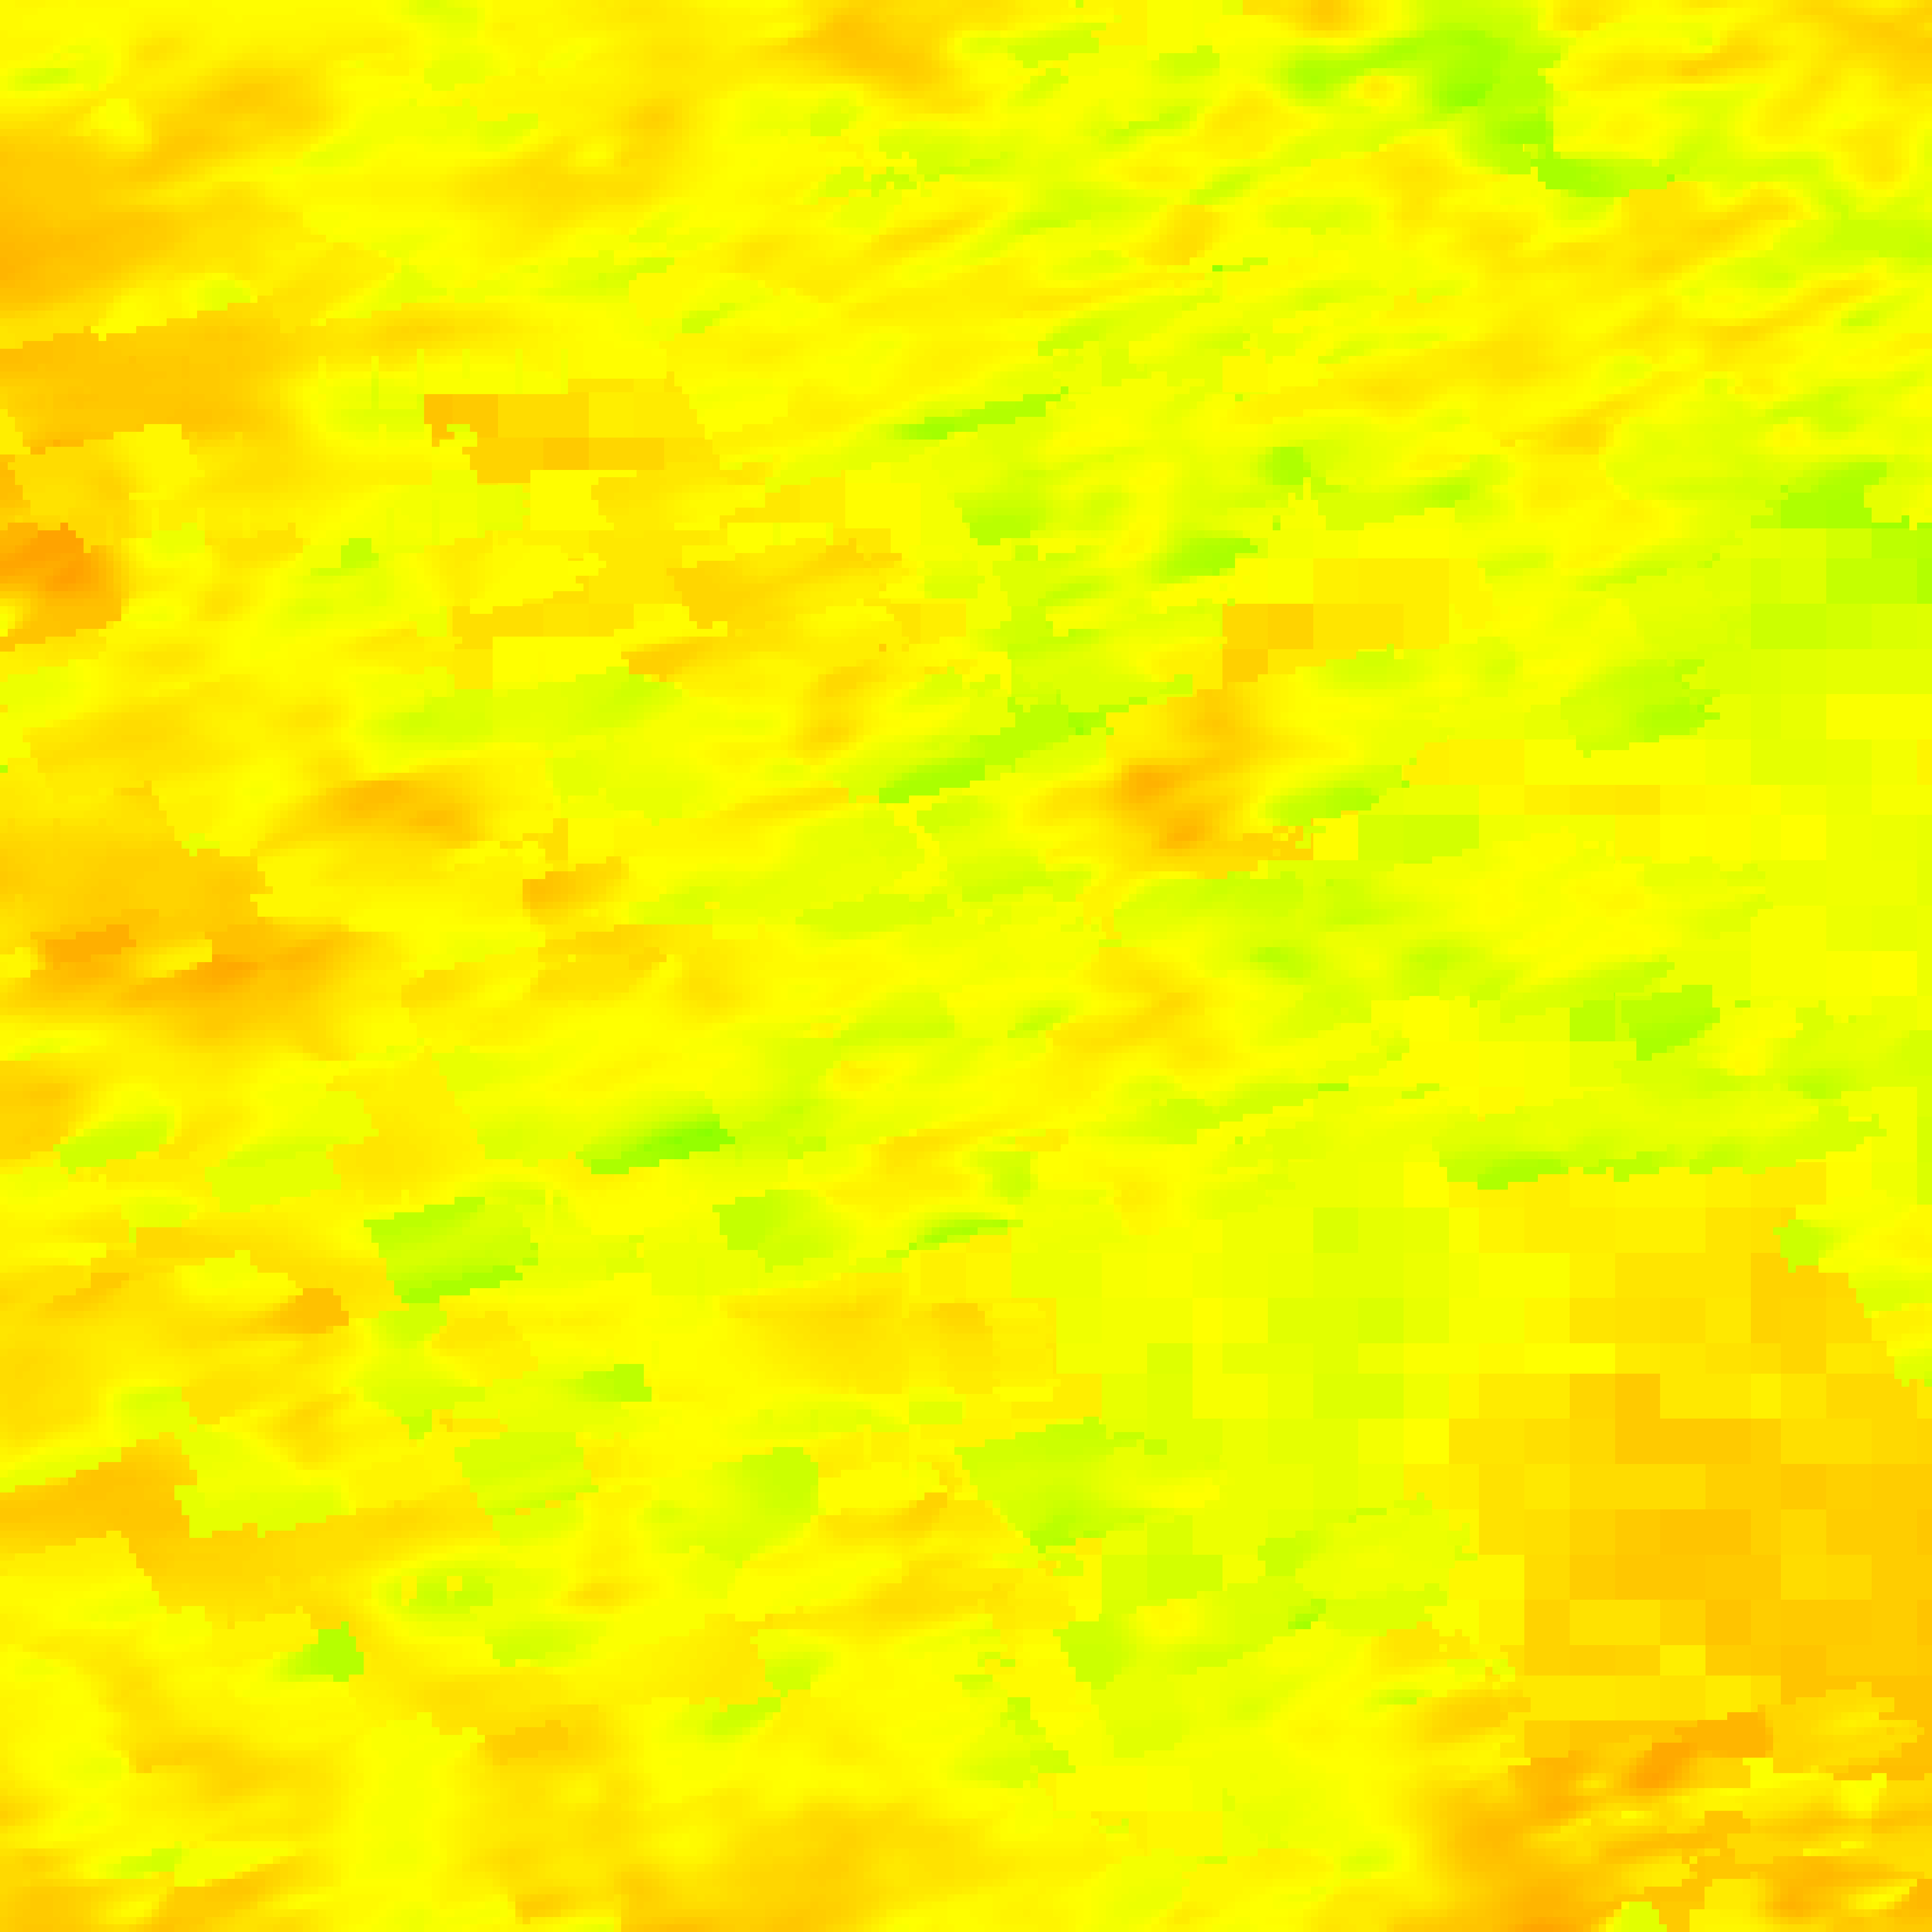
\includegraphics[width=2.5in]{download/temp/20110725.png}}
	\caption{Visualization results of Satellites}
	\label{fig:visualization_satellites}
\end{figure}

We then used drought index data from Drought Monitor, a system developed by various U.S. government agencies to monitor and report on drought conditions. The system is updated weekly and provides nationwide drought data, analysis, and monitoring, as well as warnings and recommendations for different geographic areas. We collected drought levels from 2010-2020 for each U.S. state in the Drought Levels and DSCI data for use in our model tests, as shown in the Figure \ref{fig:visualization_data}.


\begin{figure}[htb]
	\centering
	\subfigure[Forrest]{
		\includesvg[width=0.3\textwidth]{forrest.svg}
		\label{fig:forrest}
	}
	\subfigure[Grassland]{
		\includesvg[width=0.3\textwidth]{grassland.svg}
		\label{fig:grassland}
	}
	\subfigure[Dessert]{
		\includesvg[width=0.3\textwidth]{dessert.svg}
		\label{fig:dessert}
	}
	\caption{Visualization results of Drought Monitor}
	\label{fig:visualization_data}
\end{figure}


\begin{table}[htb]
	\centering
	\caption{Data set}
	\begin{tabular}{ccc}
		\toprule
		Name                 & URL                                   \\
		\midrule                                                     \\
		NASA Worldview       & https://worldview.earthdata.nasa.gov/ \\
		U.S. Drought Monitor & https://droughtmonitor.unl.edu/       \\
		\bottomrule
	\end{tabular}
	\label{tab:dataset}
\end{table}

\subsection{Data Visualization}

We represent each data item in the database as a single graph element through data visualization techniques and use the data set collected in Table \ref{tab:dataset} to form a data image while representing the individual attribute values of the data as multidimensional data, which allows for a deeper observation and analysis of the data by observing the data in different dimensions, as shown in Figure \ref{fig:way}.

\begin{figure}[htb]
	\centering
	\includesvg[width=0.8\textwidth]{way.svg}
	\caption{Data Visualization}
	\label{fig:way}
\end{figure}

Finally, we also used some data from the literature, which we have attached at the end of the paper.

\section{Model 1: Plant Community Interaction Model}

\subsection{Model Prepraration}

Plant growth is influenced by multiple factors, which can be mainly divided into external and internal factors. For external factors, the environment is usually the most dominant, while for internal factors, the widespread internal influences among species are also important. Therefore, we will study the changes in species communities in terms of interactions between species and the three factors that mainly influence climate. From this, we consider the analysis of the curvilinear pattern of changes in the three factors over time on species growth and modify the Lotka-Volterra model by weighting and multivariate linear fitting the weights obtained by the entropy weighting method with the three factors.

\subsection{Model Introduction}

A competition model for plant populations is a mathematical model used to describe the changes in numbers between plant populations due to contact. Common plant competition models include the Lotka-Volterra competition equation and the Tilman competition model.

This model uses the Lotka-Volterra competition equation, a common two-species competition model that is often used to describe predator-prey interactions, to model population changes due to contact between species. The model is based on the simple assumption that the population size of each species grows at a rate proportional to the number of individuals of that species, but that the growth rate does not decrease while the two species compete with each other to maintain a stable value. The mathematical form of the Lotka-Volterra competition equation is as follows.

\begin{align}
	\begin{aligned}
		\frac{dN_1}{dt} = r_1 N_1(1-\frac{N_1}{K_1} - \frac{a_{12}N_2}{K_1}) \\
		\frac{dN_2}{dt} = r_2 N_2(1-\frac{N_2}{K_2} - \frac{a_{21}N_1}{K_2})
	\end{aligned}
\end{align}


Where $N_1$ and $N_2$ are the numbers of individuals of the two competing species; $r_1$ and $r_2$ are the endogenous growth rates of the two species, respectively; $K_1$ and $K_2$ are the environmental capacities of the two species, respectively; and $a_{12}$ and $a_{21}$ are the competition coefficients between the two species.

The Lotka-Volterra competition model can be used to simulate population changes due to competition between different species of plants and interactions between the same species, on the basis of which future changes in plant communities can be predicted at the same time.

At the same time, the Lotka-Volterra competition model can likewise be easily extended to use in the case of n species. On the basis of the above equation, we can describe the competition among n species by the following set of differential equations:

\begin{equation}
	\frac{dN_i}{dt} = r N_i(1-\frac{N_i}{K_i} - \sum_{j=1}^n a_{ij} \frac{N_j}{K_j})
\end{equation}

Where $N_i$ is the number of individuals of the $i$th species, $r_i$ is the intrinsic growth rate of the $i$th species, $K_i$ is the environmental capacity of the $i$ th species, and $a_{ij}$ is the competition coefficient of the $j$th species against the $i$ th species. The Lotka-Volterra competition model takes into account both the environmental capacity and species relationship influences on community abundance, $\frac{N_i}{K_1}$ indicates that the specific growth rate is influenced by the environmental holding capacity $K$ and also by the relative number and competitive ability between two species. In this model, we do not consider the effects caused by the same species to grab resources and space, i.e., the survival environment and space are sufficient. Therefore, the value of $a_{ii}$ is zero here.

From the theoretical model described above, we know that there is competition between two different species for food and habitat without considering the influence caused by the external environment. In general, the difference in competitiveness between two different species is not large, and eventually, the two populations reach a relative equilibrium and maintain it stably. For two species with a large difference in species competitiveness, the usual outcome is that the more competitive one competes the relatively less competitive one to extinction, and the autochthonous one reaches the environmental capacity allowed by the ecosystem. Therefore, we can predict the subsequent course of the final two species by giving the initial values between two different species, the environmental holding capacity, and their mutual competition coefficients.

\subsubsection{Solution to the Problem 1}

The use of the Lotka-Volterra competition model is predicated on the so-called need to give initial values between two different species, the environmental accommodation, and their competition coefficients with each other in order to predict the subsequent course of the final two species. For \textbf{Problem 1}, using the present model does not give us the option to give these values. Instead, we innovatively propose an ecosystem-based competition model theory, in other words, instead of giving the number between two different species, we cleverly solve the problem that the series parameters between two different species are not easy to determine by considering the larger concept of ecosystem. By considering 2-3 unique species within the ecosystem, we successfully solve the problem of predicting the number of organisms when considering both species competition and environmental factors.

Specifically, it is assumed that only three different species exist in the ecosystem and that no other species exist in the ecosystem within a certain range, i.e., there is no interference with the model data from species other than these three. We use the observable "Vegetation Index" of the satellite species to predict the subsequent changes in biomass.

In the introduction, we have given the Lotka-Volterra competition model for $N$ species, as in Eq. Therefore, the Lotka-Volterra competition equation based on three different species can be given as follows.

\begin{equation}
	\left \{
	\begin{aligned}
		 & \frac{dp}{dt} = r_1p (1- \frac{p - \alpha (q + \mu)}{K_1})     \\
		 & \frac{dq}{dt} = r_2q (1- \frac{q - \beta (p + \mu)}{K_2})      \\
		 & \frac{d\mu}{dt} = r_3\mu (1- \frac{\mu - \gamma (p + q)}{K_3}) \\
	\end{aligned}
	\right .
\end{equation}

Where $p$, $q$, $\mu$ is the biomass of three different species, and $K_1$, $K_2$ and $K_3$ denote the environmental capacity of the three species, i.e., the maximum amount that can support the survival of the species when only species competition is considered. $r_1$, $r_2$, and $r_3$ denote the growth rates of species 1,2, and 3, respectively, and $\alpha$ beta gamma denotes the competition coefficient between the three different species. The competition coefficient between the three different species. Meanwhile, the growth inhibition of $p$, $q$, and $\mu$ populations by their own populations is $\frac{1}{k_1}$,$\frac{1}{k_2}$, $\frac{1}{k3}$ and the influence of $p$, $q$, $\mu$ populations by other populations is $\frac{a}{k_1}$, $\frac{b}{k_2}$, and $\frac{c}{k_3}$, respectively. the specific values of each parameter are shown in Table


\begin{table}[htb]
	\caption{Parameter of Lotka-Volterra model}
	\centering
	\begin{tabular}{@{}llll@{}}
		\toprule
		         & $r$ & $\frac{1}{k}$ & $p$,$q$,$\mu$ \\
		\midrule
		$\alpha$ & 0.4 & 0.005         & 0.03          \\
		$\beta$  & 0.7 & 0.008         & 0.02          \\
		$\gamma$ & 0.5 & 0.012         & 0.01          \\
		\bottomrule                                    \\
	\end{tabular}
	\label{tab:lv_parameter}
\end{table}

We can change these coefficients to alter the different growth curve relationships of species, make different species grow at different rates by adjusting the growth rate of each species, and adjust the competition coefficients between different species to show the interspecific competition relationships of different species. On the basis of the table, we can draw the biomass of the three species as a function of time, as shown in Figure \ref{tab:lv_parameter} .

\begin{figure}[htb]
	\centering
	\includesvg[width=0.5\textwidth]{population.svg}
	\caption{The biomass of three different species with respect to time}
	\label{fig:population}
\end{figure}

This figure shows the change curves of the biological population of three different species with respect to time. It can be noted that the three different species have different growth rates and upper bounds for their three curves due to their different initial numbers of species, different growth rates of species, and different competition coefficients of species. In addition, we also plotted an image of the total ecosystem biomass on top of this graph, which is the red curve in the Figure \ref{fig:population}. This is because we have used the concept of "Vegetation index" to measure the total biomass of species, as described earlier, by summing the three curves.

We collected all biomass data of Yellowstone Park from 2010 to 2020, collected the changes in biomass in the park over ten years, and plotted them in month classification. On top of this, we also superimposed the total biomass obtained from the graph with it and plotted the total biomass versus time for the theoretical model compared with the observed values as in Figure \ref{fig:predict_and_actual}.

\begin{figure}[htb]
	\centering
	\includesvg[width=0.5\textwidth]{dselta.svg}
	\caption{Predicted and actual biomass}
	\label{fig:predict_and_actual}
\end{figure}

Without considering other factors, although there are more than three species in Yellowstone, the growth trend of the total biomass should be consistent with the image obtained from the Lotka-Volterra competition model, but the fact is that the two curves do not overlap and the observed values are significantly lower than those calculated by the theory, and the model also has errors, as shown in Figure \ref{fig:error}.

\begin{figure}[htb]
	\centering
	\includesvg[width=0.5\textwidth]{error.svg}
	\caption{Errors in model prediction}
	\label{fig:error}
\end{figure}

\subsection{A Little Correction}

Although the above model can describe the species population change curve with time to some extent, it still cannot fit the data values we observed well, and there is an error value, thus indicating that there are some non-negligible factors that we accidentally ignored. Therefore, it is still necessary to correct the model we obtained on the basis of the above in order to finally obtain a predictable model image, as in Eq. where let the theoretical value of the observed total biomass be $f(t)$ and the value we actually get is $g(t)$, and there is an error $\delta$ between the two.

\begin{equation}
	f(t) = g(t) + \delta
\end{equation}

After considering the internal factors between different species, the external factors objectively brought by the environment should not be neglected as well. Therefore, the impact of the variable climatic environment on organisms in the environment should be taken into account $\delta$.

There are many factors in the environment that affect the growth of organisms, such as $CO_2$ concentration, microorganisms in the soil, and pH in rainwater, but the three most important factors for plant growth are temperature, precipitation, and sunlight, for the following reasons.

\begin{enumerate}
	\item \textbf{Temperature}: The life activities of living organisms are based on aerobic respiration, and the metabolic activities carried out by aerobic respiration require enzymes in a specific temperature range to work properly to catalyze the reactions. Too high or too low ambient temperature can affect the growth and development of the organism or even death.
	\item \textbf{Precipitation}: The life activities of living organisms are carried out with water as a carrier. Living organisms not only need water to maintain cellular functions and life activities but also need water as a carrier for information transfer and energy transport. Too much or too little water may affect the growth and development of living organisms.
	\item \textbf{Sunlight}: For plants, light is necessary for photosynthesis, and only in a place with proper and sufficient sunlight can plants properly carry out photosynthesis to release oxygen and produce organic matter.
	      Therefore, we will consider the influence of the environment on organisms from the above three factors.
\end{enumerate}

Therefore, we will consider the influence of the environment on organisms from the above three factors.

\begin{figure}
	\centering
	\includesvg[width=0.5\textwidth]{tree.svg}
	\caption{Physiological activities of plants}
	\label{fig:tree}
\end{figure}

\vspace{0.5cm}

\textbf{Temperature effects on changes in total biomass}

\vspace{0.5cm}

Temperature plays a key role in plant growth and development because many of the physiological processes that take place in plants require a certain temperature. In general, plants will grow faster at higher temperatures than at lower temperatures because the former respiration rate is higher than the latter. The photosynthesis of plants is affected by temperature, which in turn affects total biomass, and is modeled theoretically by the following equation.

\begin{equation}
	\frac{dN}{dt} = rN(1-\frac{N}{K}) - c(T-T_0)N
\end{equation}

Where $N$ denotes the population size of the plant, r is the growth rate of the plant population, K is the environmental holding capacity, c denotes the influence factor of temperature on plant growth, T is the current ambient temperature, and T0 is the baseline temperature for plant growth. The above equation is solved by MATLAB and the image is obtained as Figure \ref{fig:temp}.

\begin{figure}[htb]
	\centering
	\includesvg[width=0.5\textwidth]{temp.svg}
	\caption{Temperature and Biomass}
	\label{fig:temp}
\end{figure}

\vspace{0.5cm}

\textbf{Impact of precipitation on changes in total biomass}

\vspace{0.5cm}

Precipitation is one of the most fundamental meteorological phenomena in nature and it has a profound impact on the environment. Precipitation is one of the necessary conditions for vegetation growth, and plants need water to grow, photosynthesize and metabolize substances. Suitable precipitation can promote plant growth and increase crop yield. The changes in the total biomass of plant communities due to the influence of precipitation can be expressed as follows.

\begin{equation}
	\frac{dN}{dt} = rN (1 - \frac{N}{K} ) \frac{W} {W_0}
\end{equation}

Where $N$ is the number of individuals in the plant community, $r$ is the specific growth rate, $K$ is the environmental holding capacity, $W$ are the amount of precipitation, and $W_0 $represents the optimum rainfall level for plants, the image of which is shown in Figure \ref{fig:water}.

\begin{figure}[htb]
	\centering
	\includesvg[width=0.5\textwidth]{pre.svg}
	\caption{Precipitation and Biomass}
	\label{fig:water}
\end{figure}

It is not difficult to see from the images that the total amount of plants increases with the increase of precipitation within a certain precipitation range. However, after exceeding the optimum precipitation amount $P_0$ for plants, the total amount of plants instead decreases with the increase of precipitation.

\vspace{0.5cm}

\textbf{Effect of sunlight on changes in total biomass}

\vspace{0.5cm}

Light is also one of the key factors for plant growth because sunlight provides the necessary energy for photosynthesis, enabling plants to increase their total biomass by converting CO2 and water into organic matter, and the relationship between light and total plant mass has the differential equation.

\begin{equation}
	\frac{dN}{dt} = rN(1-\frac{N}{K})f(t)
\end{equation}

Where $N$ denotes the number of plant communities, $r$ denotes the growth rate of plants, $K$ denotes the capacity of the ecosystem, and $f(t)$ denotes the variation of light intensity at time $t$. In the real situation, the variation of light is repeated in small cycles of one day and large cycles of one year. To simplify our model, we can choose a simple periodic function to replace the variation of light intensity, such as a simple sine function.

\begin{equation}
	f(t) = \sin(\omega t)
\end{equation}

\begin{figure}[htb]
	\centering
	\includesvg[width=0.5\textwidth]{sunlight.svg}
	\caption{Sunlight and Biomass}
	\label{fig:sunlight}
\end{figure}

\vspace{0.5cm}

\textbf{The Entropy Weight Method}

\vspace{0.5cm}

From the above description we can know that in the actual environment, sunlight, precipitation, and temperature generally speaking influence the growth of total biomass by affecting the photosynthesis of plants and thus the growth of total biomass, but these factors affect different proportions of the same. Based on the need to determine the weights of multiple indicators, we decided to evaluate the influence of each index on the correction value in a comprehensive way by the entropy weight method.

The entropy weighting method is a commonly used method to determine the weights of multiple indicators. By calculating the relative entropy values between multiple indicators, we can quickly and accurately calculate the weighting relationships between different indicators without a priori results, so as to improve the accuracy of the results. For the determined index, we need to calculate the entropy value $E_i$ of the $i$th index, i.e.

\begin{equation}
	E_i = - \frac{1}{ln(n)} \sum_{j=1}^n \frac{p_{ij}}{ln(p_{ij})}
\end{equation}

Where $n$ denotes the number of indicators, $p_{ij}$ denotes the proportion of the $i$th indicator in the $j$th sample, and $\ln$ denotes the natural logarithm. Then, the weight $w_i$ of each indicator is calculated based on the entropy value of the indicator.

\begin{equation}
	\hat{w_i} = \frac{w_i}{\sum^n_{i=1}w_i}
\end{equation}

The weights of the obtained indicators are normalized so that the sum is equal to 1

\begin{equation}
	w_i = \frac{1 - E_i}{n - \sum^n_{j=1} E_j}
\end{equation}

Based on the above description, we analyzed all the data of sunlight, precipitation, and temperature changes in Yellowstone Park during 2010-2020 using the entropy weighting method to determine the weights. The calculation results are as follows Figure \ref{fig:pie}

\begin{figure}[htb]
	\centering
	\includesvg[width=0.55\textwidth]{pie.svg}
	\caption{Weighting ratio of the three factors}
	\label{fig:pie}
\end{figure}

\vspace{0.5cm}

\textbf{Solution}

\vspace{0.5cm}

We obtained the relationship between the effects of temperature, precipitation, and light on total plant biomass. Then, we obtained the corresponding weights of the three variables by analyzing these three data. Next, we need to consider these three together and use them to correct our model.

Multiple linear fitting is a statistical analysis method used to analyze the relationship between multiple independent variables and a dependent variable. Through multiple linear fitting, we can determine the degree of influence of the independent variables on the dependent variable and use the fitted results to make predictions or interpretations, the general equation of the multiple linear regression equation is as follows.

\begin{equation}
	y_i =  b_1  x_{i1} + b_2  x_{i2} + \cdots + b_n  x_{in} + e_i
\end{equation}

The three weights obtained above were then used to perform a multivariate linear fit to them, and the actual error values were approximated by least squares tests and minimizing the sum of squares of the residuals. For the three factors of temperature, precipitation, and light, the following linear regression equations are available.

\begin{equation}
	\delta = \zeta x_1 + \eta x_2 + \xi x_n + \epsilon
\end{equation}

By solving and fitting their values, the parameter values of $\zeta$, $ \eta$, $\xi$, and $\epsilon$ are tabulated in Table \ref{tab:fitting}.

\begin{table}[htb]
	\centering
	\caption{Fitting Parameter values}
	\begin{tabular}{@{}llll@{}}
		\toprule                                \\
		$\zeta$ & $\eta$  & $\xi$  & $\epsilon$ \\
		\midrule                                \\
		0.34119 & 1.70569 & 0.5320 & 1.0962     \\
		\bottomrule                             \\
	\end{tabular}
	\label{tab:fitting}
\end{table}

\begin{equation}
	\delta = 0.34119 x_1 + 1.70569 x_2 + 0.5320 x_n + 1.0962
\end{equation}

As a result, we obtained the Lotka-Volterra competition model based on the multiple regression entropy methods, which can provide a good prediction of species numbers in relation to time after correcting for errors by taking into account the effects of species exchange and environmental factors, given sunlight, precipitation, and temperature parameters in advance, and the number of species over a period of time.

\section{Model 2: Plant Community Interaction Environment Model}

Unlike Model 1, we selected three different ecosystems under the same climatic conditions as the subject of this model (in this model it is a temperate monsoon climate). Since we selected ecosystems with the same climatic conditions. Therefore, we do not consider the effects of sunlight, precipitation, and temperature due to climate in the model. For a single species in an ecosystem, the number of species is continuous over time and has a constant growth rate in the absolute ideal case. We can derive the one-dimensional differential equation for the number of species with respect to time as follows.

\begin{equation}
	\frac{dN(t)}{dt} = cN(t)
\end{equation}

Where $c$ denotes the growth rate of the species. However, all of the above is possible only under ideal conditions, considering that the number of organisms that the environment can bear, i.e., the environmental holding capacity, is limited within a certain range of the community. According to the Logistic growth principle, the growth rate of a species population slowly decreases with time due to the limited environmental carrying capacity. Therefore, we consider the blocking factor $\frac{1-N(t)}{k}$ that affects the number of species and correct the equation to

\begin{equation}
	\frac{dN(t)}{dt} = cN(1 - \frac{N}{K})
\end{equation}

\subsection{Solution to the Problem 4}

Although the subjects we selected for the study are all in the same environment, i.e., for the effects brought about by climate the three are equivalent in time scale, in other words, the effects on the number of species are equivalent. However, in the case of extreme drought, the growth rate of organisms is likely to decrease or even stop due to the lack of water resources. Therefore, taking into account the influence of irregular weather conditions in the environment, and under the assumption that the influence of environmental factors and interspecific relationships on community biomass is linear, we derive the following equation.

\begin{equation}
	\frac{dN(t)}{dt} = rN(t)(1-\frac{N(t)}{K} - \alpha D)
\end{equation}

This equation is compared with Eq. with an additional coefficient $\alpha D$. where $\alpha$ is the effect of environmental factors on community biomass, and since $\alpha$ is only a coefficient controlling the degree of drought impact, we can temporarily ignore the effect of changes in this value. d is the drought index. At this point, the number of species is not only limited by the environmental holding capacity $K$ but also affected by irregular drought conditions. We use the Drought Monitor's drought index to measure the drought conditions of the area. This drought index is obtained from the cumulative drought monitoring data, i.e., the percentages of D0 to D4 for a given week are summed to obtain the drought severity and coverage index for that week.

Thus, we can get the answer to question four. For more frequent and more variable droughts. An increase in drought frequency increases the effect of drought on plant community biomass by affecting the magnitude of $\alpha$, while greater variability affects the change in plant community biomass by climatically changing the value of the drought index $D$.

\subsection{Solution to the Problem 3}

Although the coefficient aD presented in question four takes into account the more frequent and variable drought climate scenario, the biomass in relation to time differs in our chosen study population, even though the effects of drought on the three ecosystems are simultaneous and equivalent. The Figure \ref{fig:three} shows the total biomass of three ecosystems, namely forest, grassland, and desert, obtained after fitting processing.

\begin{figure}[htb]
	\centering
	\includesvg[width=0.5\textwidth]{3.svg}
	\caption{Total biomass of three ecosystems}
	\label{fig:three}
\end{figure}

The graph is a plot of total biomass versus time for three ecosystems, namely forest, grassland, and desert, obtained after fitting processing. From the figure, it can be concluded that the growth rate of the three curves varies without considering the influence of climate and other factors, and the speed of their growth rate is determined by the inherent properties of their ecosystems. For different organisms, the curves grow faster in the initial period when the biomass is low. However, the growth rate of the curve slows down due to the influence of environmental capacity. As can be seen from the figure, the three curves do not overlap and have a certain distance.

Therefore, we add a coefficient $\beta$ to the above equation and define it as the "Species Contact Coefficient". The so-called species contact coefficient is essentially the coefficient of the difference in the number of species between ecosystems, specifically the effect of interspecific relationships between species on the biomass of the community. This coefficient defines the relationship between species and the sum of the values of harmful and beneficial exposures between species.

\begin{equation}
	\frac{dN(t)}{dt} = rN(t)(1-\frac{N(t)}{K} - \alpha D+ \beta)
\end{equation}

The answer to question 3 is that, given the same environmental factors, differences in species types affect the growth of total biomass by influencing what we define as the "species contact factor". As the number of species increases, their biomass grows faster and faster over time, and the gradient of growth becomes larger and larger.

\subsection{Solution to the Problem 2}

The differential equations of forest community biomass for different environmental factors and interspecific relationships can be evolved accordingly for the community biomass for different environmental factors and interspecific relationships under grassland, and desert regions, as follows.

\begin{equation}
	\left .
	\begin{aligned}
		 & \frac{dN_1(t)}{dt} = r_1N_1(t)(1-\frac{N_1(t)}{K_1} - \alpha D_1 + \beta_1) \\
		 & \frac{dN_2(t)}{dt} = r_2N_2(t)(1-\frac{N_2(t)}{K_2} - \alpha D_2 + \beta_2) \\
		 & \frac{dN_3(t)}{dt} = r_3N_3(t)(1-\frac{N_3(t)}{K_3} - \alpha D_3 + \beta_3)
	\end{aligned}
	\right .
\end{equation}

Where $N_1$, $N_2$, and $N_3$ represent the biomass of forest, grassland, and desert, respectively; $r_1$, $r_2$, and $r_3$ represent the growth rates of species 1,2, and 3, respectively; $a$, $b$, and $c$ represent the interspecific competition coefficients, respectively; and $k1$, $k_2$, and $k_3$ represent the maximum environmental holding capacity of species, respectively.

We chose the grassland ecosystem as a benchmark and made the following scatter plot of its biomass with respect to time and fitted it as a function, as shown in Figure \ref{fig:biomass}.

\begin{figure}[htb]
	\centering
	\includesvg[width=0.5\textwidth]{biomass.svg}
	\caption{Grassland ecosystem biomass}
	\label{fig:biomass}
\end{figure}

By fitting the function and comparing it with our theoretical model, we can derive the difference $\delta$, which is the value of the "species contact coefficient" mentioned in the previous section, which is only related to the species of the community ecosystem, but not to the environment and other factors.

Similarly, for the other two ecosystems, we can obtain the "species contact coefficients" for the three different ecosystems, as shown in the Table \ref{tab:contact}.


\begin{table}[htb]
	\centering
	\caption{Species contact coefficients}
	\begin{tabular}{@{}lll@{}}
		\toprule                       \\
		Forrest & Grasslands & Dessert \\
		\midrule                       \\
		0.025   & 0.017      & 0.008   \\
		\bottomrule
	\end{tabular}
	\label{tab:contact}
\end{table}

We next focus on the issue of ecosystem benefit, which for plant communities benefits the community in several ways.

\begin{enumerate}
	\item \textbf{Photosynthesis}: Through photosynthesis, plants absorb carbon dioxide from the air and emit oxygen back to the atmosphere, maintaining the carbon cycle and oxygen balance of the ecosphere.
	\item \textbf{Provision of food}: As the bottom producer in the biosphere, plants have the function of transferring energy and providing food to the upper layers of the food chain. Through photosynthesis, plant bodies obtain energy from sunlight and transfer it to higher consumers within the food chain.
	\item \textbf{Habitat}: Some large plants can also provide habitat and protection functions for some small animals. The shading of sunlight by large trees and the range of their influence make animals protected.
	\item \textbf{Maintain soil structure and prevent erosion}: Plants have very well-developed root systems, which penetrate deep into the ground to maintain the soil structure and prevent erosion and erosion caused by rainfall.
\end{enumerate}

We used two parameters, Fraction of Photosynthetically Active Radiation and Gross Primary Productivity, to evaluate the impact on the ecosystem.

The fraction of Photosynthetically Active Radiation is the proportion of radiant energy in the visible spectrum in the range of 400-700 nm to the full wavelength of radiant energy, which can be absorbed by pigments such as chlorophyll and converted into chemical energy, thus promoting photosynthesis in plants and thus increasing their oxygen production. Primary Productivity is the rate at which an organism converts inorganic substances into organic substances through photosynthesis or chemical synthesis in an ecosystem over a certain period of time. These organic substances supply the organism's own energy and nutrient needs and support the survival of other organisms in the ecosystem.

Therefore, based on the above elaboration, it is reasonable for us to use these two data to determine the impact of the community on the ecosystem.

\begin{figure}[htb]
	\centering
	\subfigure[Fraction of Photosynthetically Active Radiation]{
		\includesvg[width=0.4\textwidth]{fraction.svg}
	}
	\subfigure[Gross Primary Productivity]{
		\includesvg[width=0.4\textwidth]{Productivity.svg}
	}
	\caption{Two parameters of ecosystem impact}
\end{figure}

Since the periodicity of the images can be clearly observed for the above two variables, we first classify them, i.e., by month for the years 2010-2020, and perform a linear fit to the above two variables, using the slope $k$ of their functions as their return coefficients.

\begin{figure}[htb]
	\centering
	\includesvg[width=0.5\textwidth]{slope1.svg}
	\caption{Fited of Funciton}
	\label{fig:slope1}
\end{figure}

Similarly, the species exposure coefficients for the three ecosystems and their benefit coefficients can be calculated as Table \ref{tab:factor}.

\begin{table}[]
	\centering
	\caption{Species Exposure Factor and Benefit Factor}

	\begin{tabular}{@{}ll@{}}
		\toprule
		Species exposure factor & Benefit factor \\
		\midrule                                 \\
		0.025                   & 0.06704        \\
		0.017                   & 0.04451        \\
		0.008                   & 0.01524        \\
		\bottomrule                              \\
	\end{tabular}
	\label{tab:factor}
\end{table}

The analytical equation can be derived from the above equation

\begin{equation}
	y = 3.051x - 0.02858
\end{equation}

When $y = 0$, we have $x = 0.00937$

That is when its species contact coefficient is 0.00937, the coefficient of the benefit of the population to the ecosystem is 0. At this point, the species contact coefficient is 1.17125 times the species contact coefficient of the grassland, and according to mentioned, the grassland has an average of 393 different species \cite{wang2017biogeographic}, so we can conclude that the minimum number of species that benefit the community is 460 species.

The equation we derived here also further proves that in Problem 4: When greater frequency and wider variation of the occurrence of droughts, their rainfall will decrease. Since the independent variable b is positively correlated with the response variable y. Therefore, the greater frequency and wider variation of the occurrence of droughts will decrease. Therefore, the greater frequency and wider variation of the occurrence of droughts will also lead to a decrease in species biomass.

\subsection{Solution to Problem 5}

The three questions above all explore the relationship between community biomass and time well without considering external factors, but real life is not so rosy. In addition to the effects of natural factors on biomass, human-caused impacts have more serious effects on plants. For example air pollution, dust pollution, toxins, crop diseases, etc.

For less severe impacts, we consider that such impacts are different from the previously mentioned environmental drought, and although they also reduce total biomass, the rate of reduction should be exponentially increasing.

In the equation, $P$ represents the negative effect of environmental pollution on total biomass. This indicates that organisms are very sensitive to pollution, implying that a very small amount of pollution can be devastating to an entire biome or even cause the extinction of a specific species.

\section{Sensitive Analysis}

Considering that differences in the number of species types differ in the extent to which they are beneficial to the environment, we wanted to test the sensitivity of the model by performing a sensitivity analysis of the second problem using a second model. Based on the above study, we consider that the species exposure coefficient increases at 5\% to obtain a set of control curves, from which it is calculated that

\begin{figure}
	\centering
	\subfigure{\includesvg[width=0.4\textwidth]{slope2.svg}}
	\subfigure{\includesvg[width=0.4\textwidth]{slope.svg}}
	\caption{Sensitivity Analysis}
\end{figure}

From the data in the figure, it can be concluded that the benefit coefficient changes sensitively as the species exposure coefficient increases.

\section{Discussion}

\subsection{Solution to Problem 6}

\begin{figure}[htb]
	\centering
	\includesvg[width=1\textwidth]{mind.svg}
	\caption{Flowchart of the model}
	\label{fig:flowchart}
\end{figure}

According to the flowchart, abnormal weather cycles have a double impact on the diversity of plant tribes. On the one hand, if plant tribes become more diverse, the competition between different plant species will become more intense and therefore the number of each species will decrease, which has a negative impact on plant diversity. On the other hand, biodiversity will certainly increase the stability of the ecosystem. When unusual weather cycles occur, ecosystems with high biodiversity are more likely to maintain reproductive efficiency and avoid collapse.

The importance of biodiversity is different in different environments. Arid environments prefer low plant diversity because in this case, the environment is stable, so maintaining efficient reproduction is a priority. As plant tribal diversity increases, it becomes more important to maintain the stability of the system, and therefore, in forest environments, plant tribal diversity is high.

\subsection{Strengths}

\begin{itemize}
	\item Our model is based on a certain theoretical foundation. By reviewing a large amount of literature, the corresponding parameters were selected. For the model solution, it can be found that it fits well with the real values, which shows that our model can predict the changes in plant populations under abnormal weather conditions more accurately.
	\item Since nature is full of unknowns, we made a reasonable simplification by selecting among the climatic factors the more influential cases of temperature, precipitation, and light on plants. We used the forest scenario to predict, and then we calculated the grassland and desert, and we tested the accuracy of the model, which can reflect the universality of our model to some extent.
	\item We verified the stability of the model through reasonable assumptions and sensitivity analysis of the model.
\end{itemize}

\subsection{Weaknesses}

\begin{itemize}
	\item The growth rate of the same species is not constant due to environmental changes and human factors, and this paper does not analyze the growth rate of such changes.
	\item Nature is a chaotic system, and there are many uncontrollable factors in nature, such as severe weather conditions that we cannot predict.
\end{itemize}

\subsection{Futher Work}

In this paper, we only selected the study in the United States, the climate of drought areas around the world is not necessarily the same, so we should select a larger research scope to study, and in the future, we can propose better models or more advanced algorithms to expand the model to more objects with a wider range of application.

\bibliography{bibfile}
\bibliographystyle{plain}
%%%%%%%%%%%%%%%%%%%%%%%%%%%%%%
\end{document}
\end